\documentclass[letterpaper, 10 pt, journal, twoside]{IEEEtran}  % Comment this line out if you need a4paper

%\documentclass[a4paper, 10pt, conference]{ieeeconf}      % Use this line for a4 paper

\IEEEoverridecommandlockouts                              % This command is only needed if 
% you want to use the \thanks command

%\overrideIEEEmargins                                      % Needed to meet printer requirements.
\usepackage{multirow}
\usepackage[utf8]{inputenc}
\usepackage{amsmath}
\usepackage{amsfonts}
\usepackage{amssymb}
\usepackage{graphicx}
\usepackage{amsmath}
\usepackage{float}
\usepackage{placeins} %table position
\usepackage{cite}
\usepackage{url}
\usepackage{verbatim}
\usepackage{algorithm,tabularx}
\usepackage[noend]{algpseudocode}
%\usepackage{subfigure}
\usepackage{caption}
\usepackage{adjustbox}
\usepackage{booktabs}
\usepackage{subcaption}
\makeatletter
\newcommand{\multiline}[1]{%
	\begin{tabularx}{\dimexpr\linewidth-\ALG@thistlm}[t]{@{}X@{}}
		#1
	\end{tabularx}
}
\makeatother


\title{Model-Free 6D Pose Estimation via Geometric Representation Refinement: A Low-Light Benchmark}

	

\begin{document}		
	\maketitle	
	\begin{abstract}
	
Model-free 6D object pose estimation enables generalization to unseen objects but remains highly sensitive to degraded geometric observations, particularly under low-light conditions where depth sensing becomes noisy and incomplete. Inaccurate geometry leads to unstable coarse pose initialization and degraded pose accuracy.
We propose a geometric representation refinement framework that improves model-free 6D pose estimation by enhancing coarse alignment without modifying or retraining the underlying networks. The proposed approach decouples object geometry into core and boundary regions and performs view-aware, region-specific refinement to suppress outliers while preserving structural consistency. Furthermore, a minimal oriented bounding box initialization strategy is introduced to  stabilizes coarse alignment and alleviates scale ambiguity caused by partial observations.
To enable systematic evaluation under controlled illumination degradation, we introduce LL6DPose, a large-scale synthetic dataset designed for low-light 6D pose estimation. The dataset simulates realistic lighting variations and sensor artifacts that are difficult to capture and annotate reliably in real environments. Extensive experiments demonstrate consistent improvements across multiple datasets, showing that the proposed framework serves as a plug-and-play enhancement for robust 6D pose estimation under challenging lighting conditions.

\end{abstract}
	\begin{IEEEkeywords}
	6D Pose Estimation, Geometric Representation, Low-Light Vision, Benchmark
	\end{IEEEkeywords}

\IEEEpeerreviewmaketitle
  \section{Introduction}


\IEEEPARstart{O}{bject} 6D pose estimation aims to estimate the 3D translation and 3D orientation of objects from sensory observations, such as RGB-D images or point clouds. Accurate 6D pose estimation is a critical component in many robotic applications, including grasping \cite{gumeli2023objectmatch}, manipulation \cite{an2024rgbmanip}, augmented reality \cite{wang2024nerfs}, and autonomous navigation \cite{zou2021end}. Traditional approaches typically rely on object-specific 3D models, which restrict their applicability in dynamic environments characterized by diverse scenes and viewpoints. By eliminating the requirement for prior CAD models, these methods enable pose prediction for previously unseen objects and significantly improve generalization in open-world robotic scenarios \cite{he2022fs6d}.

\begin{figure}[htb]
	\centering
	% 子图 (a): anchor
	\begin{subfigure}[b]{0.45\linewidth}
		\centering
		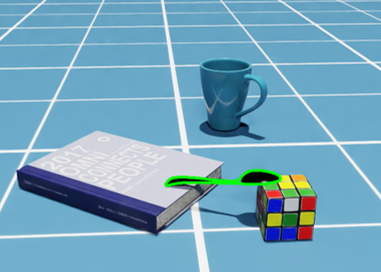
\includegraphics[width=\linewidth]{1_1}
		\caption{Anchor Image}
		\label{anchor}
	\end{subfigure}
	\hfill
	% 子图 (b): 正常光照
	\begin{subfigure}[b]{0.45\linewidth}
		\centering
		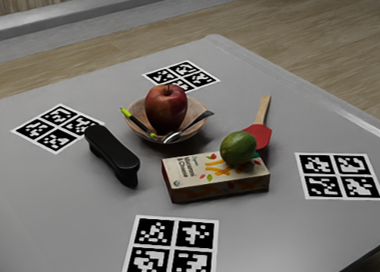
\includegraphics[width=\linewidth]{1_2}
		\caption{Normal illumination}
		\label{normal light}
	\end{subfigure}
	
	\vspace{0.5cm} % 行间间距
	
	% 子图 (c): point cloud
	\begin{subfigure}[b]{0.45\linewidth}
		\centering
		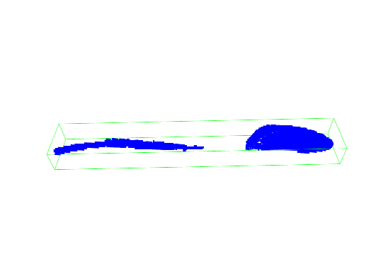
\includegraphics[width=\linewidth]{1_3}
		\caption{point cloud}
		\label{point cloud}
	\end{subfigure}
	\hfill
	% 子图 (d): pose
	\begin{subfigure}[b]{0.45\linewidth}
		\centering
		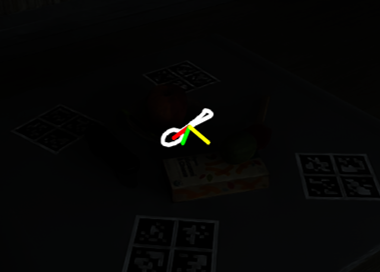
\includegraphics[width=\linewidth]{1_4}
		\caption{6D Object Pose}
		\label{pose}
	\end{subfigure}
	
	\caption{Comprehensive comparisons between our method and .... (a) ...our method achieve better performance than ....on the various object pose estimation datasets.}
	\label{fig.1}
\end{figure}
% 这个图主要展示方法效果

Existing model-free 6D pose estimation methods, such as Any6D \cite{lee2025any6d}, have demonstrated impressive performance on novel objects without requiring object-specific CAD models. Despite this progress, their effectiveness remains heavily dependent on the reliability of geometric observations used for coarse pose initialization. In practical robotic scenarios, geometric inputs derived from partial viewpoints and noisy depth sensing frequently suffer from outliers, missing regions, and structural distortions. Such degradations lead to unstable pose initialization, which subsequently undermine the accuracy of downstream refinement.


Similar limitations are also observed in correspondence-based pipelines. For example, OnePose++ \cite{he2022onepose++} relies on structure-from-motion (SfM) for object modeling and 2D–3D matching for pose estimation. FS6D \cite{he2022fs6d} which extends this paradigm to RGB-D inputs, depends heavily on reliable feature correspondences. However, these correspondences become increasingly fragile under adverse lighting conditions, particularly in low-light environments, where color cues are weak and object boundaries are difficult to perceive. As a result, unreliable geometric observations fundamentally limit the robustness and generalization of existing pose estimation systems.

Since retraining or redesigning existing frameworks is often impractical due to their general-purpose nature and deployment constraints, there is a critical need for a plug-and-play geometric refinement framework that enhances geometric reliability and stabilizes pose estimation without modifying the underlying networks. Motivated by this insight, we propose a geometry-centric refinement framework that enhances geometric reliability in a plug-and-play manner without modifying existing pose estimation networks. The proposed method improves coarse alignment through view-aware core–boundary decomposition and region-specific outlier filtering, while a minimal oriented bounding box (OBB) initialization stabilizes alignment and alleviates scale ambiguity, providing a reliable starting point for downstream pose estimation, as shown in Fig. \ref{fig1}


To systematically evaluate 6D pose estimation under challenging lighting conditions, we further construct Dark6D, a large-scale synthetic benchmark featuring diverse object geometries, multi-object scenes, and low lighting  effects that are difficult to capture and annotate in real environments. The dataset enables controlled evaluation of geometric refinement strategies and provides a standardized benchmark for future work in low-light pose estimation.

Overall, this work improves the robustness of 6D pose estimation by enhancing the reliability of geometric representations rather than redesigning pose estimation architectures, enabling consistent performance gains across diverse datasets. Project page is publicly available at \url{https://yhldrf.github.io/pointcloudchange/}. The primary contributions of this work are summarized as follows:


\begin{itemize}\itemsep0pt
	\item \textbf{View-Aware Geometric Representation Refinement:}  	We propose a view-aware refinement framework that improves object geometry reliability under partial observations and noisy depth. By decoupling point clouds into core and boundary regions and applying region-adaptive filtering, our method suppresses outliers while preserving structural consistency, enhancing pose stability without requiring network retraining.
	\item \textbf{Robust Initialization with Minimal Oriented Bounding Box:}  We introduce a minimal oriented bounding box-based initialization strategy to mitigate scale ambiguity and improve alignment stability under incomplete observations, providing a reliable geometric prior for downstream pose estimation and optimization.
	
	\item \textbf{LL6DPose Benchmark:}  	We construct a large-scale synthetic dataset featuring diverse illumination, multi-object scenes, and realistic sensor degradation. LL6DPose enables systematic evaluation of pose estimation robustness under low-light scenarios that are typically difficult to capture and annotate in real environments.
\end{itemize}



 \section{Previous work}
 \subsection{Model-Free Object Pose Estimation}
 In recent years, 6D object pose estimation has advanced beyond the reliance on CAD models, leading to the emergence of model-free approaches. 
 Early works such as Gen6D~\cite{liu2022gen6d} and OnePose~\cite{sun2022onepose} and its extension OnePose++~\cite{he2022onepose++} eliminate the need for explicit 3D models by leveraging single-view observations or keypoint-free strategies for pose estimation. 
 However, these methods often rely on multi-view reconstruction to build object-level 3D representations, which limits their accuracy under restricted viewpoints, severe occlusions, or noisy environments.
 
 Subsequent approaches aim to improve practicality by reducing reliance on multi-view data. 
 Methods such as SamPose~\cite{shi2025sampose} and AxisPose~\cite{zou2026axispose} propose generalizable single-view frameworks, enabling more efficient inference without complex preprocessing or matching pipelines. 
 Nevertheless, purely vision-based representations remain sensitive to heavy occlusions and cluttered backgrounds, which degrade robustness and generalization.
 
 Recent efforts further explore model-free generalization under limited supervision. 
 FS6D~\cite{he2022fs6d} and NOPE~\cite focus on few-shot or single-view settings to reduce data collection costs, while LoFTR~\cite{sun2021loftr} leverages transformer-based feature matching to improve robustness in pose estimation. 
 However, these approaches still struggle under severe occlusions. 
 GigaPose~\cite{nguyen2024gigapose} estimates object pose via image-to-3D alignment but requires rendered templates to infer object scale. 
 GFreeDet~\cite{liu2024gfreedet} introduces Gaussian splatting and large-scale visual representations for model-free detection, yet its performance degrades in complex environments. 
 FoundationPose~\citen{wen2024foundationpose} unifies pose estimation and tracking within a single framework, and Any6D~\cite{lee2025any6d} further improves generalization without explicit model dependence.
 
 Despite these advances, existing methods remain sensitive to degraded geometric observations. 
 In particular, noisy point clouds and severe occlusions significantly affect geometric consistency, leading to unstable pose estimation. 
 This limitation is especially pronounced in low-light conditions, where sensor noise further deteriorates depth quality.
 \begin{table}[htbp]
 	\caption{Comparison of 6D object pose detection datasets.}
 	\centering
 	\renewcommand{\arraystretch}{1.2}
 	\resizebox{\linewidth}{!}{
 		\begin{tabular}{lccccccc}
 			\toprule
 			\textbf{Dataset}   & \textbf{Modality} & \textbf{Multi-object} & \textbf{Occlusion} & \textbf{Low-light} & \textbf{Scene Complexity} & \textbf{Synthetic} \\
 			\midrule
 			LINEMOD        & RGB-D & $\times$ & $\checkmark$ & $\times$ & Simple      & $\times$ \\
 			LM-O           & RGB-D & $\times$ & $\checkmark$ & $\times$ & Moderate    & $\times$ \\
 			YCB-Video      & RGB-D & $\checkmark$ & $\checkmark$ & $\times$ & Complex     & $\times$ \\
 			REAL275        & RGB-D & $\checkmark$ & $\checkmark$ & $\times$ & Complex     & $\times$ \\
 			YCB-LFOAT      & RGB-D & $\checkmark$ & $\checkmark$ & $\times$ & Complex     & $\times$ \\
 			T-LESS         & RGB-D & $\checkmark$ & $\checkmark$ & $\times$ & Industrial  & $\times$ \\
 			IC-BIN         & RGB-D & $\checkmark$ & $\checkmark$ & $\times$ & Industrial  & $\times$ \\
 			CAMERA25       & RGB-D & $\checkmark$ & $\checkmark$ & $\times$ & Moderate    & $\checkmark$ \\
 			Toyota Light   & RGB-D & $\times$ & $\times$ & $\checkmark$ & Simple       & $\times$ \\
 			FAT            & RGB-D & $\checkmark$ & $\checkmark$ & $\times$ & Moderate    & $\checkmark$ \\
 			Ours           & RGB-D & $\checkmark$ & $\checkmark$ & $\checkmark$ & Complex    & $\checkmark$ \\
 			\bottomrule
 		\end{tabular}
 	}
 	\label{table_dataset_comparison}
 \end{table}
 
   \begin{figure*}[ht]
 	\centering
 	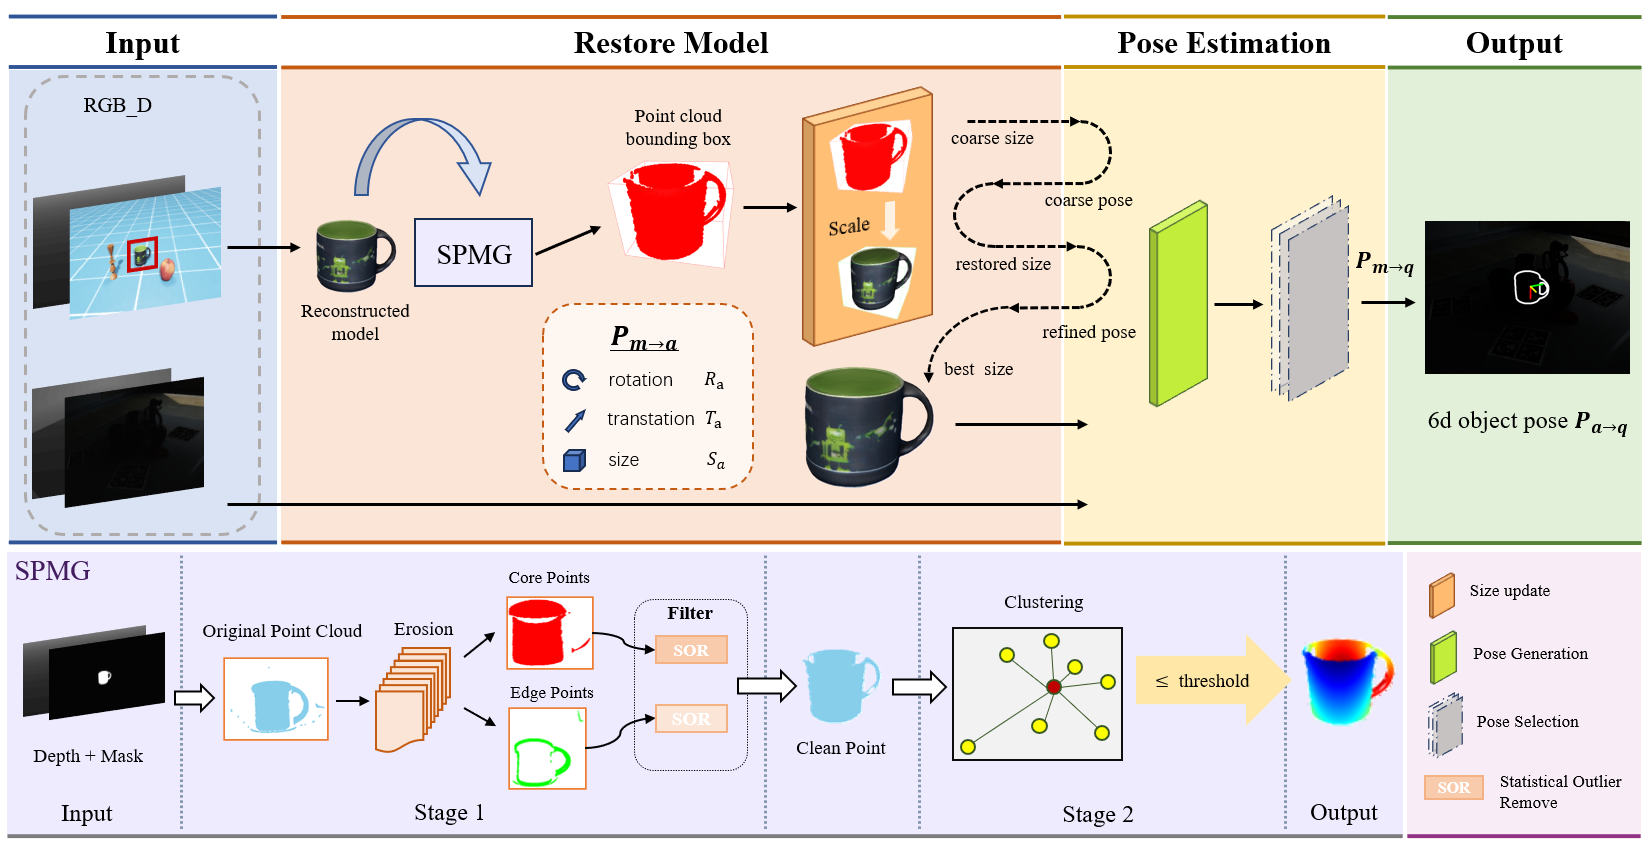
\includegraphics[width=1\textwidth]{pipeline}
 	\caption{the overall pipeline of the proposed method.The object model is first reconstructed from the anchor image. 
 		With the proposed SPMG module, noisy point clouds are refined into high-quality geometric representations. A bounding box is then estimated from the filtered point cloud and used to rescale the reconstructed model, recovering its physical scale. 
 		Meanwhile, the pose of the anchor image is estimated using the FoundationPose~\cite{wen2024foundationpose} framework.Subsequently, the pose of the query image is estimated using the same pose estimation method. By combining the two poses, the relative 6D pose between the anchor and query images is obtained.}
 	\label{Fig. 2}
 \end{figure*}
 
 \subsection{6D Object Pose Estimation Datasets}
 High-quality datasets play a crucial role in advancing 6D object pose estimation. 
 Most existing benchmarks, such as LINEMOD~\cite{hinterstoisser2012model}, YCB-Video~\cite{xiang2017posecnn}, T-LESS~\citen{hodan2017t}, LM-O~\cite{brachmann2014learning}, REAL275~\cite{wang2019normalized}, and IC-BIN~\cite{kleeberger2019large}, adopt RGB-D inputs and provide accurate pose annotations by aligning depth observations with CAD models. 
 These datasets achieve high precision under controlled environments, but are typically captured under stable lighting conditions and limited scene complexity, making them insufficient to reflect real-world challenges.
 
 To increase task difficulty, several datasets introduce specific variations. 
 YCBInEOAT~\cite{wen2020se} and REAL275~\cite{wang2019normalized} incorporate multi-object scenes with severe occlusions, while T-LESS emphasizes texture-less objects, highlighting the importance of geometric cues. 
 CAMERA25~\cite{lee2021category} combines synthetic and real data to improve generalization. 
 However, these datasets are predominantly collected under normal or well-lit conditions and lack systematic modeling of visual degradation caused by low-light environments.
 More recently, Toyota Light~\cite{hodan2018bop} focuses on varying illumination conditions, but primarily considers single-object scenarios and lacks complex multi-object interactions and occlusions. 
 Synthetic datasets such as Falling Things~\cite{fallingthings} provide large-scale data with diverse poses and physical interactions, benefiting training and evaluation, yet still exhibit a gap in realism compared to real-world scenes.
 Overall, existing datasets tend to address only a single aspect of the problem, such as occlusion, texture, or illumination. 
 There remains a lack of a unified benchmark that simultaneously captures low-light conditions, multi-object interactions, and complex environmental disturbances.

\section{Methodology}
  \subsection{Overview}
  In this work, we perform object pose estimation based on the Any6D framework. 
  Given an RGB-D anchor image, a normalized object model is constructed. 
  The scale of the reconstructed model is then recovered using a bounding box estimated from the point cloud, while obtaining the pose $P_{m \rightarrow a}$. 
  The recovered model is further used to estimate the pose $P_{m \rightarrow q}$ for a given query image. 
  By combining these two poses, the relative 6D pose $P_{a \rightarrow q}$ is obtained.
  The relative transformation $P_{a \rightarrow q}$ is defined as a rigid transformation $[\mathbf{R} \mid \mathbf{t}]$, where $\mathbf{R} \in \mathrm{SO}(3)$ denotes the rotation matrix and $\mathbf{t} \in \mathbb{R}^3$ denotes the translation vector.
  
  Although the original pipeline provides a strong solution for 6D object pose estimation, its performance remains sensitive to noisy depth observations, particularly during the object scale reconstruction stage.
  To address this limitation, we introduce two key modifications in the geometric preprocessing stage: 1) a region-partitioned statistical filtering method for robust point cloud denoising, and 2) a minimal oriented bounding box estimation for more accurate geometric initialization.
  After obtaining a clean and structurally consistent point cloud, we replace the conventional  oriented bounding box estimation with a minimal oriented bounding box, which yields a tighter geometric enclosure of the object. By enhancing the accuracy of object-scale reconstruction, the proposed method facilitates more accurate and efficient downstream pose estimation.
  \subsection{Pose Initialization}
  \textbf{Geometry-aware representation refinement}    
  In low-light environments, depth observations are often corrupted by sensor noise, resulting in significant outliers in the reconstructed point cloud. Conventional statistical filtering methods tend to treat all points uniformly, which may lead to excessive removal of structural points near object boundaries. To address this issue, we propose a Structure-Preserving Point Cloud Filtering that leverages object segmentation priors and local density statistics to achieve robust and structure-preserving point cloud filtering, as shown in Fig.2
  
  Given an input point cloud $\mathcal{P} = \{ \mathbf{p}_i \in \mathbb{R}^3 \}$ reconstructed from the depth map and the corresponding binary object mask $M \subset \mathbb{R}^2$, each 3D point is projected onto the image plane using the camera intrinsic matrix $\mathbf{K}$:
  \begin{equation}
  	(u_i, v_i) = \pi(\mathbf{p}_i) = \mathbf{K} \mathbf{p}_i
  \end{equation}
  where $\pi(\cdot)$ denotes the projection function.
  
  To preserve structural integrity while removing noise, the mask $M$ is decomposed into two regions via morphological operations:
  \begin{align}
  	M_c &= \mathrm{Erode}(M, r) \\
  	M_e &= M \setminus M_c
  \end{align}
  where $r$ denotes the structuring element radius. The core region $M_c$ represents stable interior areas, while the edge region $M_e$ corresponds to object boundaries.
  Each point is then classified according to its projected location:
  \[
  \mathbf{p}_i \in 
  \begin{cases}
  	\text{Core region}\ p_c, & (u_i, v_i) \in M_c \\
  	\text{Edge region}\ p_e, & (u_i, v_i) \in M_e \\
  	\text{Background}, & \text{otherwise}
  \end{cases}
  \]
  Points projected outside the mask are directly discarded. For the remaining points, Statistical Outlier Removal (SOR) is applied separately to the core and edge regions. The SOR method evaluates the average distance between a point and its $k$-nearest neighbors.
  
  To balance noise removal and structure preservation, different thresholds are used for the two regions:
  \begin{equation}
  	\mathbf{p}_i \in
  	\begin{cases}
  		\text{inlier}, & d_i \leq \mu + \alpha_c \sigma, \quad \mathbf{p}_i \in p_c \\
  		\text{inlier}, & d_i \leq \mu + \alpha_e \sigma, \quad \mathbf{p}_i \in p_e \\
  		\text{outlier}, & \text{otherwise}
  	\end{cases}
  \end{equation}
  where $d_i$ denotes the mean distance of point $\mathbf{p}_i$ to its $k$-nearest neighbors, $\mu$ and $\sigma$ represent the mean and standard deviation of $\{d_i\}$ over the point set, respectively. $\alpha_c < \alpha_e$ enforces stricter filtering in the core region and relaxed filtering in the edge region.
  
  Although Region-Partitioned Statistical Filtering removes most obvious outliers, isolated sparse points may still remain. Therefore, we introduce a density-adaptive filtering stage based on robust statistics.
  Given the filtered point set $\mathcal{P} = \{ \mathbf{p}_i \}$, we define the local density measure for each point as the mean distance to its $k$-nearest neighbors:
  \begin{equation}
  	d_i = \frac{1}{k} \sum_{\mathbf{p}_j \in \mathcal{N}_k(\mathbf{p}_i)} \left\| \mathbf{p}_i - \mathbf{p}_j \right\|_2
  \end{equation}
  Instead of using standard deviation, which is sensitive to extreme values, we employ the Median Absolute Deviation (MAD) for robust estimation:
  \begin{align}
  	m &= \mathrm{median}(d_i) \\
  	\mathrm{MAD} &= \mathrm{median} \left( \left| d_i - m \right| \right)
  \end{align}
  The adaptive filtering threshold is defined as
  \[
  T = m + \lambda \frac{\text{MAD}}{0.6745}
  \]
  where $\lambda$ is a tunable parameter controlling the filtering strength.
  Points satisfying are retained, while points with significantly larger neighbor distances are considered sparse outliers and removed.
  \[
  d_i \leq T
  \]
  
  This two-stage filtering framework effectively combines semantic priors from object masks and robust density statistics, enabling reliable removal of noisy points while preserving important geometric structures.
  
  \textbf{Robust Initialization via Minimal OBB}    
  Accurate object scale estimation requires a reliable object center and a tightly fitted bounding box. 
  Although the axis-aligned bounding box (AABB) is simple, it often yields inaccurate centers and poor geometric alignment. 
  Oriented bounding box (OBB), typically obtained via principal component analysis (PCA), improve alignment with the underlying point distribution. 
  Nevertheless, PCA-based OBB can still produce suboptimal fits for irregular shapes or partial observations.
  To address this, we adopt minimal oriented bounding box(MOBB), yielding tighter geometric fits and more stable pose estimation.
  
  \begin{figure}[htbp]
  	\centering
  	% 子图 (a): 原始点云中心
  	\begin{subfigure}[b]{0.45\linewidth}
  		\centering
  		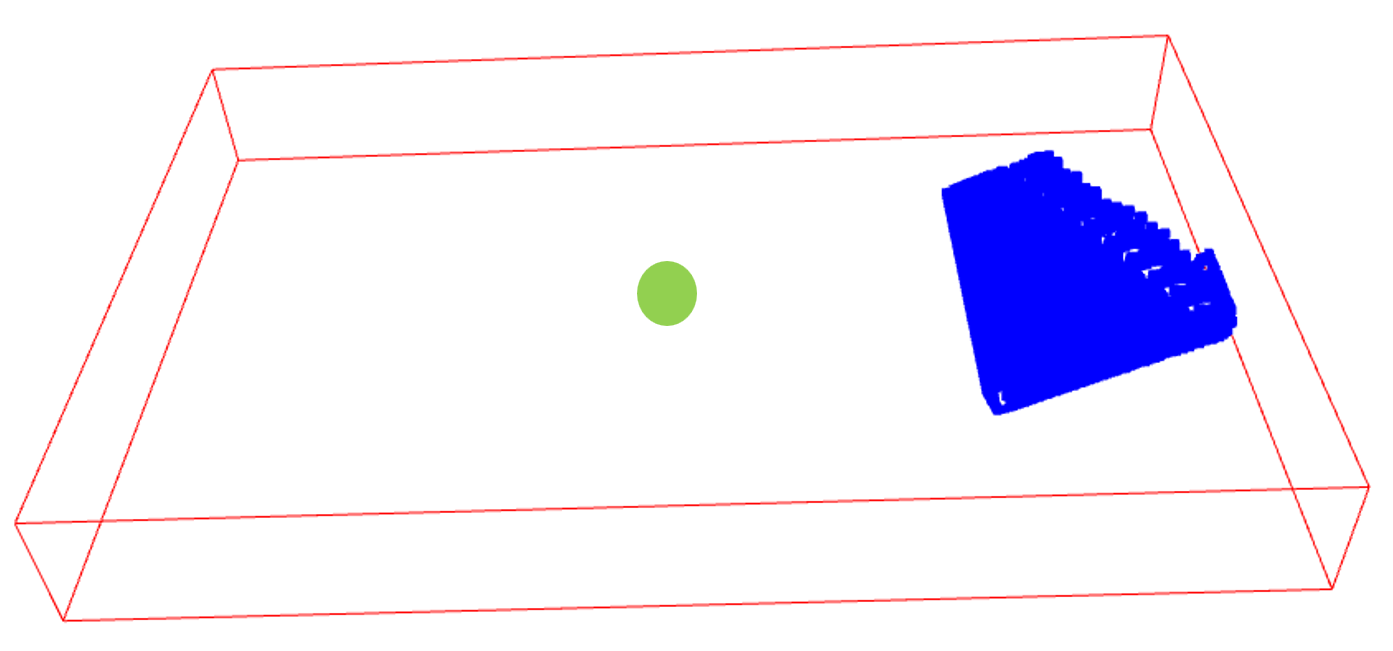
\includegraphics[width=\linewidth]{3_1}
  		\caption{Center of Raw Point Cloud}
  		\label{fig:raw}
  	\end{subfigure}
  	\hfill
  	% 子图 (b): 滤波后点云中心
  	\begin{subfigure}[b]{0.45\linewidth}
  		\centering
  		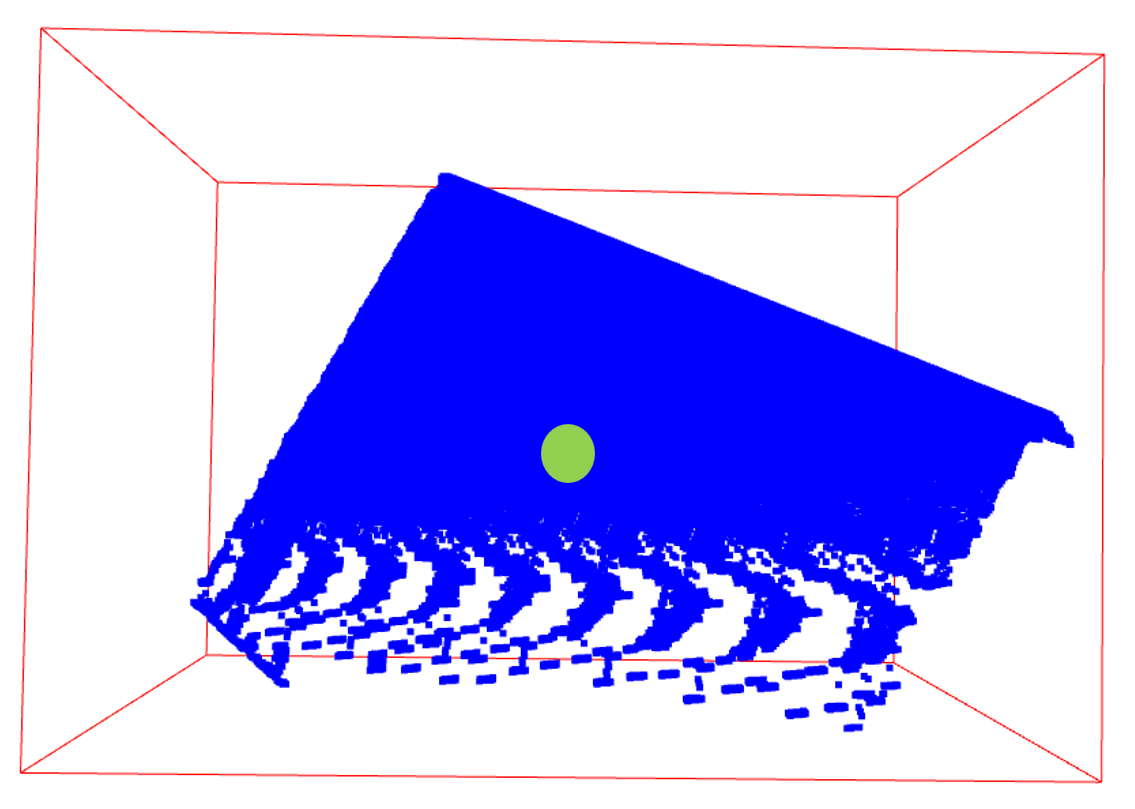
\includegraphics[width=\linewidth]{3_2}
  		\caption{Center of Bounding Box of Filtered Points}
  		\label{fig:filtered}
  	\end{subfigure}
  	
  	\vspace{0.5cm} % 行间间距
  	
  	% 子图 (c): 滤波点云的轴对齐包围盒中心
  	\begin{subfigure}[b]{0.45\linewidth}
  		\centering
  		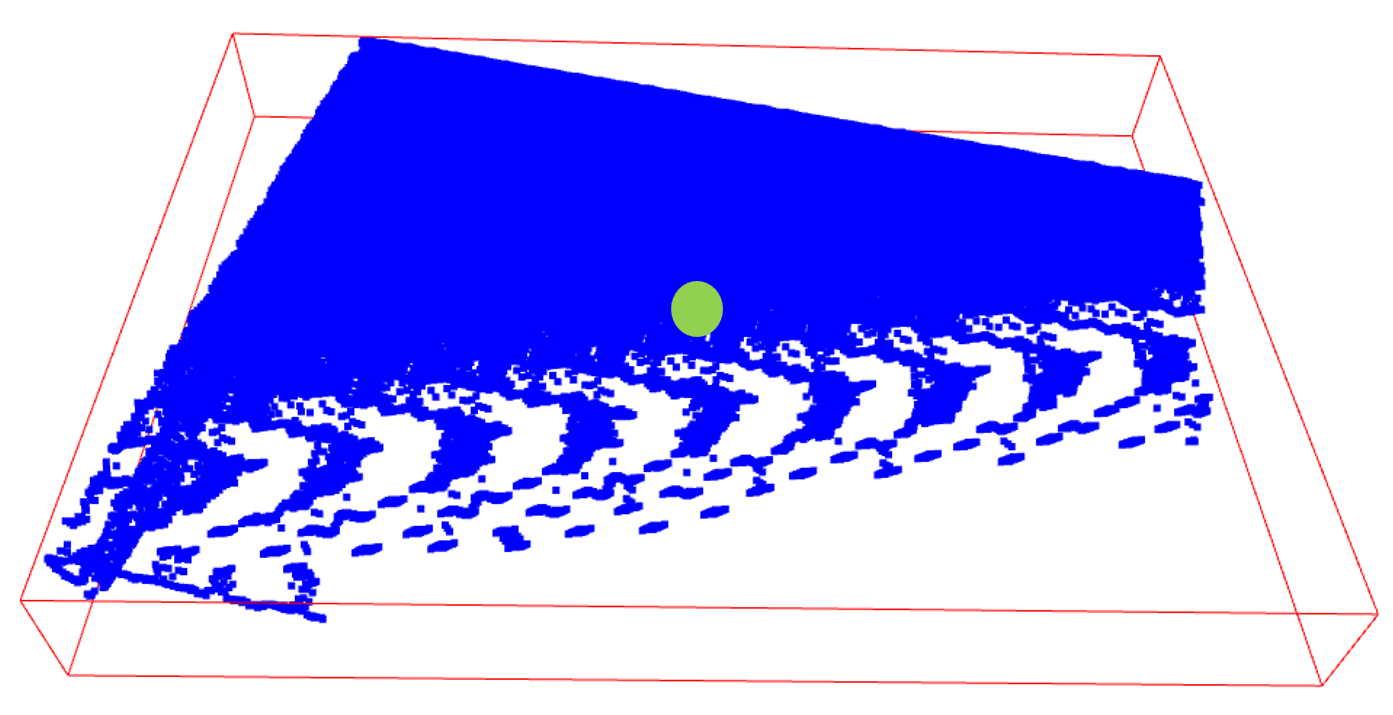
\includegraphics[width=\linewidth]{3_3}
  		\caption{Center of Oriented Bounding Box of Filtered Points}
  		\label{fig:aabb}
  	\end{subfigure}
  	\hfill
  	% 子图 (d): 滤波点云的定向包围盒中心
  	\begin{subfigure}[b]{0.45\linewidth}
  		\centering
  		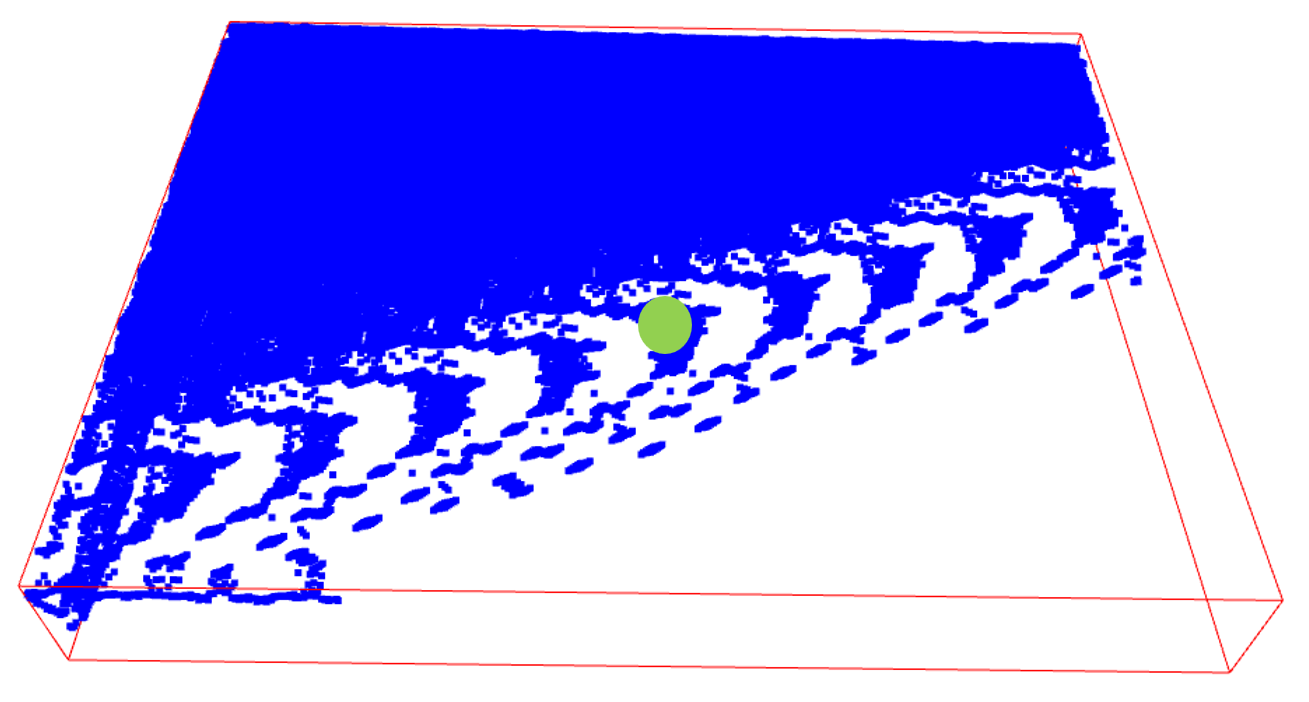
\includegraphics[width=\linewidth]{3_4}
  		\caption{Center of Minimal Oriented Bounding Box of Filtered Points}
  		\label{fig:obb}
  	\end{subfigure}
  	
  	\caption{Visualization of each point clouds}
  	\label{pointcloud_centers}
  \end{figure}
  
  \subsection{Pose Refinement}
 
\section{LL6DPose Benchmark}

To enrich existing datasets, we construct a virtual dataset for 6D object pose estimation, with a focus on low-light conditions, multi-object interactions, and complex environmental disturbances. 
The dataset is developed using the NVIDIA Isaac Sim platform, enabling a high-quality and controllable data generation pipeline.

\textbf{Design.} 
We select 20 object categories with diverse shapes and surface properties, including spheres, cuboids, and irregular structures. 
These objects cover both highly textured instances and texture-less surfaces, enhancing the diversity of visual characteristics. 
To better simulate real-world scenarios, objects are manually arranged with varying positions and orientations, and complex occlusion patterns are intentionally introduced. 
As a result, multiple objects exhibit mutual occlusions and partial overlaps across different frames. 
This design increases dataset diversity and difficulty, while effectively reflecting the challenges of object recognition and pose estimation in practical environments.

\textbf{Generation.} 
The data generation process is fully automated using Python scripts, ensuring consistency and reproducibility. 
A fixed random seed is used to control stochastic factors such as object placement and camera poses, enabling comparable samples under normal lighting conditions. 
Each object is assigned a unique category label to provide accurate semantic annotations. 
After scene initialization, cameras are automatically generated using the Replicator module to capture images from multiple viewpoints, supporting downstream 3D vision tasks.

During data collection, images are rendered at a resolution of $640 \times 480$, resulting in a total of 60,000 samples, including both low-light and corresponding normal-light images. 
To increase diversity, camera positions are uniformly sampled within a predefined range while always focusing on the scene center. 
For each frame, multiple modalities are recorded, including RGB images, segmentation masks, depth maps, and pose annotations. 
The resulting dataset enriches appearance variations and multi-view observations, providing a solid foundation for object recognition and pose estimation.

\begin{table*}[ht]
	\caption{Model-free pose estimation results measured by AUC of ADD, and ADD-S, AR on Dark6D dataset.}
	\centering
	\resizebox{\textwidth}{!}{
		\begin{tabular}{c|cccc|cccc|cccc}
			\hline
			& \multicolumn{4}{c|}{loftr} & \multicolumn{4}{c|}{Any6D} & \multicolumn{4}{c}{Ours} \\
			\cline{2-13}
			\hline
			Metrics 
			& ADD-S & ADD & AR & VSD & ADD-S & ADD & AR & VSD & ADD-S & ADD & AR & VSD \\
			\hline
			1  & 24.1 & 23.9 & 29.5 & 11.8 & 98.7 & 18.7 & 93.3 & 88.2 & 97.3 & 5.3  & 95.3 & 91.8 \\
			2  & 22.5 & 22.2 & 31.4 & 15.8 & 88.7 & 32.7 & 44.4 & 58.6 & 96   & 42   & 50.9 & 63.7 \\
			3  & 28.5 & 21.5 & 28.0 & 10.9 & 100  & 70.7 & 77.2 & 88   & 98   & 67.3 & 74.3 & 88   \\
			4  & 21.9 & 19.5 & 21.4 & 7.5  & 100  & 56   & 64.8 & 82.5 & 100  & 74   & 72.4 & 76.4 \\
			5  & 11.1 & 8.8  & 11.8 & 4.1  & 46.7 & 4    & 15.1 & 29.3 & 94   & 45.3 & 49.4 & 66.4 \\
			6  & 26.1 & 24.7 & 25.7 & 15.2 & 6    & 0    & 1.4  & 2    & 76.7 & 34.7 & 42.7 & 55   \\
			7  & 17.5 & 13.1 & 21.4 & 5.4  & 100  & 5.3  & 36.2 & 78.1 & 100  & 5.3  & 30.4 & 67.9 \\
			8  & 23.5 & 21.7 & 26.1 & 12.8 & 97.3 & 62   & 67.5 & 69.7 & 100  & 48   & 70.3 & 83.1 \\
			9  & 20.9 & 18.3 & 20.7 & 7.8  & 99.3 & 4.7  & 26.9 & 63.5 & 99.3 & 0    & 21.3 & 60.2 \\
			10 & 32.4 & 22.7 & 29.1 & 9.8  & 97.3 & 95.3 & 81.9 & 63   & 98.7 & 96.7 & 74.2 & 49.3 \\
			11 & 12.7 & 11.0 & 12.5 & 8.2  & 35.3 & 0    & 23.5 & 32   & 69.3 & 0.7  & 37.1 & 59.6 \\
			12 & 18.3 & 14.6 & 20.4 & 11.2 & 76.7 & 12   & 43   & 44.8 & 80.7 & 16   & 45.2 & 47.7 \\
			13 & 10.6 & 9.6  & 13.2 & 3.4  & 96   & 3.3  & 36.9 & 60.4 & 95.3 & 10.7 & 40   & 73.5 \\
			14 & 17.1 & 15.5 & 17.1 & 11.1 & 100  & 28   & 45.1 & 66.1 & 100  & 22   & 40.6 & 69.9 \\
			15 & 22.9 & 21.4 & 23.0 & 13.7 & 100  & 4.7  & 32.3 & 64.9 & 100  & 12   & 43.9 & 86   \\
			16 & 21.8 & 20.9 & 21.6 & 16.2 & 50.7 & 11.3 & 23.6 & 0.6  & 76.7 & 59.3 & 54.9 & 24.4 \\
			17 & 19.8 & 16.7 & 19.7 & 8.4  & 68.7 & 56.7 & 53.5 & 53.6 & 96.7 & 53.3 & 55.3 & 57.3 \\
			18 & 18.7 & 16.0 & 19.5 & 10.5 & 94.7 & 3.3  & 54.3 & 16.4 & 95.3 & 10.7 & 40   & 73.5 \\
			19 & 24.1 & 23.7 & 25.0 & 18.8 & 88   & 32.7 & 39.2 & 27.4 & 89.3 & 30.7 & 43.2 & 32.6 \\
			20 & 22.5 & 22.3 & 22.8 & 14.3 & 95.3 & 85.3 & 56.5 & 53.6 & 94.7 & 82.7 & 46.6 & 56.5 \\
			\hline
			MEAN & 20.9 & 18.4 & 22.2 & 10.8 & 82.0 & 29.4 & 44.4 & 52.3 & \textbf{91.6} & \textbf{37.3} & \textbf{52.1} & \textbf{63.4} \\
			\hline
		\end{tabular}
	}
	\label{tab:results}
\end{table*}
\section{Experiments}
\subsection{Datasets}
We evaluate our method on three benchmark datasets: HO3D, Toyota-Light, and our newly introduced Dark6D, which together cover a wide range of challenges in 6D object pose estimation.
\\ \textbf{Dark6D.}     We have constructed a new dataset called Dark6D, which contains 20 objects with diverse geometries and textures. The low-light images, captured in a virtual environment, feature multiple objects coexisting with high occlusion rates, presenting various challenges for pose estimation. The dataset includes RGB images, depth maps, occlusion maps, and pose information.
The dataset is captured in a virtual environment, providing aligned RGB images, depth maps, and segmentation masks. Example instances from Dark6D are shown in Fig. X.
\\ \textbf{HO3D}\cite{hampali2020honnotate}\textbf{.}     We further evaluate on the HO3D dataset, which provides accurate 3D pose annotations for hand-object interaction scenarios with significant mutual occlusions. Following the evaluation protocol of Any6D\cite{lee2025any6d}, we conduct experiments on a subset of 2K images for fair comparison.
\\ \textbf{Toyota-Light}\cite{hodan2018bop}\textbf{.}  The Toyota-Light dataset introduces challenging illumination variations across different scenes. It contains 21 objects and 1,659 images. Following the standard protocol, we evaluate our method on randomly sampled image pairs to assess robustness under varying lighting conditions.
\subsection{Metrics}
We adopt standard metrics in 6D pose estimation, including ADD~\cite{xiang2017posecnn,wang2019densefusion}, ADD-S, AUC, AR, MSSD, MSPD, and VSD, following the BOP evaluation protocol~\cite{hodan2024bop}.
\\ \textbf{ADD.} The Average Distance of Model Points (ADD) computes the mean distance between model points transformed by the predicted pose $[\mathbf{R}, \mathbf{T}]$ and the ground-truth pose $[\mathbf{R'}, \mathbf{T'}]$:
	\begin{equation}
		\text{ADD} = \frac{1}{N} \sum_{\mathbf{x} \in N} \left\| (\mathbf{R}\mathbf{x} + \mathbf{T}) - (\mathbf{R'}\mathbf{x} + \mathbf{T'}) \right\|
	\end{equation}
	where $N$ denotes the number of 3D model points.
\\ \textbf{ADD-S.}     For symmetric objects, ADD-S replaces the correspondence with the closest point distance:
	\begin{equation}
		\text{ADD-S} = \frac{1}{N} \sum_{\mathbf{x}_1 \in N} \min_{\mathbf{x}_2 \in N} \left\| (\mathbf{R}\mathbf{x}_1 + \mathbf{T}) - (\mathbf{R'}\mathbf{x}_2 + \mathbf{T'}) \right\|
	\end{equation}
This formulation alleviates ambiguity caused by object symmetries.
\\ \textbf{AUC and AR.}    We report the Area Under the Curve (AUC) of ADD-S errors and the Average Recall (AR) over multiple thresholds, providing a comprehensive evaluation across different error tolerances.
\\ \textbf{MSSD and MSPD.}    We further adopt BOP metrics including Maximum Symmetry-Aware Surface Distance (MSSD) and Maximum Symmetry-Aware Projection Distance (MSPD), which measure geometric and projection alignment while accounting for object symmetries.
\\ \textbf{VSD.}    The Visible Surface Discrepancy (VSD) evaluates pose accuracy based on visible surface alignment, making it robust to occlusions and truncations.

\subsection{Experimental implementation}
The overall pipeline is illustrated in Fig.~2. 
In the model recovery stage, the number of erosion iterations is set to 8, and the filtering thresholds for the core and edge regions are set to 2.5 and 3.0, respectively. 
In the pose estimation stage, we adopt the pretrained estimation network from FoundationPose. 
Therefore, the proposed method does not require any training.

 \begin{figure*}[ht]
	\centering
	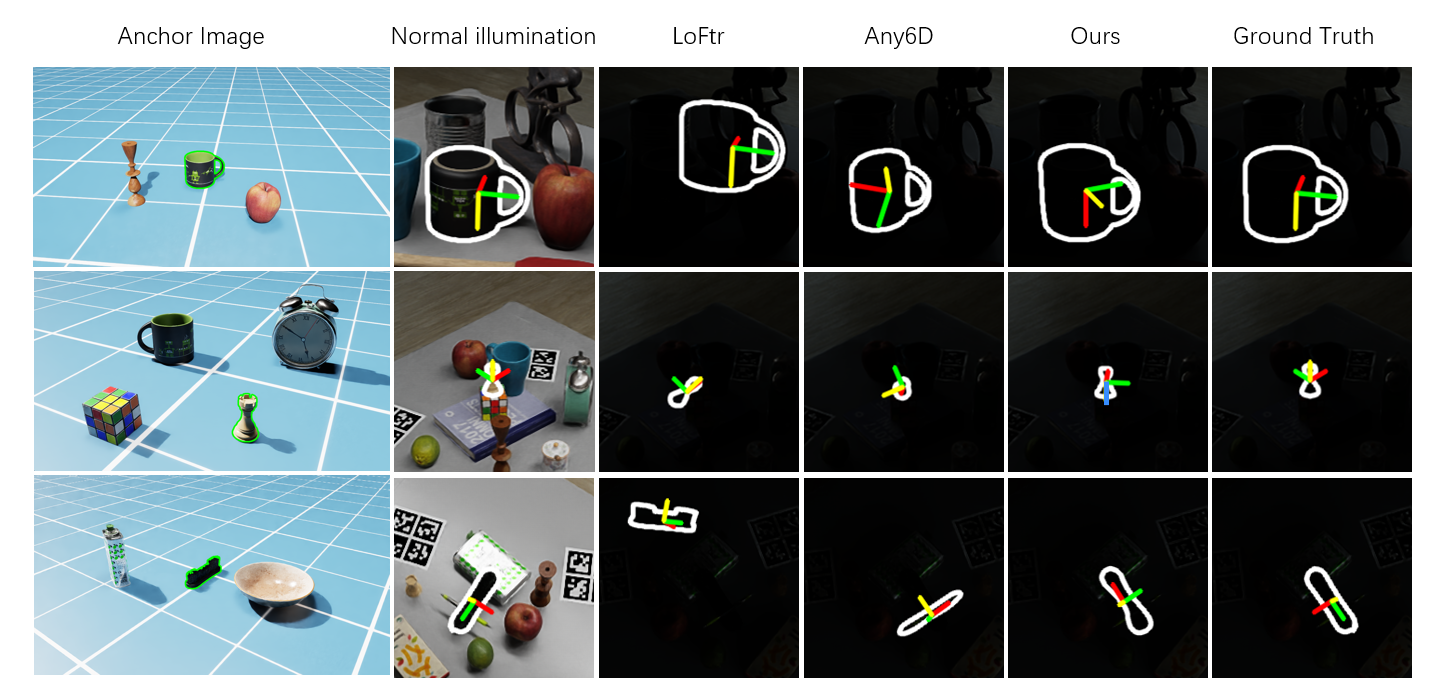
\includegraphics[width=1\textwidth]{Algorithm Comparison}
	\caption{Qualitative comparison of different methods on the Dark6D dataset. 
		The reconstructed models are projected back onto the image using the predicted poses. 
		Compared with LoFTR and Any6D, our method produces more accurate pose estimations. 
		For better visualization, we also provide images under normal lighting conditions.}
	\label{Fig. 3}
\end{figure*}

\subsection{Comparison with State-of-the-Art}
In the experiments, we evaluate our method on three challenging datasets: HO3D, Toyota-Light, and Dark6D. 
Following the evaluation protocol of Any6D, we align the relative pose $P_{a \rightarrow q}$ with the object pose $P_{m \rightarrow q}$ by multiplying with $P_{m \rightarrow a}$ during evaluation. 
We compare our method with several state-of-the-art approaches, including the multi-modal pose estimation method Oryon~\cite{corsetti2024open}, as well as single-image matching baselines such as LoFTR~\cite{sun2021loftr} and Gedi~\cite{poiesi2022learning}.

Table~2 summarizes the results on the Dark6D dataset. 
Our method significantly outperforms the compared methods, including LoFTR and Any6D, across all evaluation metrics, demonstrating superior overall performance and robustness. 
On average, our method achieves 91.6, 37.3, 52.1, and 63.4 in ADD-S, ADD, AR, and VSD, respectively, which shows clear improvements over Any6D (82.0, 29.4, 44.4, 52.3) and LoFTR (20.9, 18.4, 22.2, 10.8). 
Qualitative results are shown in Fig.~3, highlighting key observations.

On the HO3D dataset (Table~3), our method achieves superior overall performance compared to existing methods. 
In terms of ADD-S, our method achieves 96.7, which is comparable to Any6D (98.7), indicating competitive performance in overall pose accuracy. 
For the more challenging ADD and AR metrics, our method achieves 47.9 and 50.8, respectively, significantly outperforming Any6D (40.4 and 38.3) as well as other baselines such as Gedi and LoFTR. 
These results demonstrate the effectiveness and robustness of our method in complex scenarios.

On the Toyota-Light dataset (Table~4), our method outperforms all compared methods across all metrics, demonstrating stronger overall performance. 
Specifically, our method achieves 93.0 and 45.0 in ADD-S and AR, respectively, significantly surpassing Any6D (74.0 and 38.5). 
These results indicate that our method remains effective and robust under varying lighting conditions, achieving a better balance between accuracy and stability.
\begin{table}[htbp]
	\caption{Model-free pose estimation results measured by AUC of ADD, and ADD-S, AR on HO3D dataset.}
	\centering
	\resizebox{0.8\linewidth}{!}{
	\begin{tabular}{lccc}
		\hline
		Method & ADD-S & ADD & AR \\
		\hline
		Oryon   & 23.0 & 0.0  & 1.0   \\
		LoFTR   & 29.5 & 2.3  & 3.2   \\
		Gedi    & 71.9 & 9.7  & 7.4   \\
		Any6D   & \textbf{98.7} & 40.4 & 38.3 \\
		ours    & 96.7 & \textbf{47.9} & \textbf{50.8} \\
		\hline
	\end{tabular}
	}
	\label{3.results_HO3D}
\end{table}
\begin{table}[htbp]
	\caption{Model-free pose estimation results measured by AUC of ADD(S), AR, MSSD, MSPD, and VSD on the Toyota-Light dataset.}
	\centering
	\resizebox{\linewidth}{!}{
	\begin{tabular}{lccccc}
		\hline
		Method & ADD-S & AR & MSSD & MSPD & VSD \\
		\hline
		SIFT   & 14.1 & 30.3 & 39.6 & 44.1 & 7.3  \\
		Oryon  & 22.9 & 34.1 & 42.9 & 45.5 & 13.9 \\
		Any6D  & 74.0 & 38.5 & 32.9 & 35.7 & 46.9 \\
		ours   & \textbf{93.0} & \textbf{45.0} & \textbf{36.3} & \textbf{40.2} & \textbf{58.6} \\
		\hline
	\end{tabular}
	}
	\label{4.results_tyol}
\end{table}

\begin{table}[htbp]
	\caption{Ablation study of different modules.}
	\centering
	\resizebox{\linewidth}{!}{
	\begin{tabular}{lccccccc}
		\hline
		method   & RF & DF & MOBB & ADD-S & ADD & AR \\
		\hline
		baseline & $\times$ & $\times$ & $\times$ & 82.0 & 29.4 & 44.4 \\
		A        & $\times$ & $\times$ & $\times$ & 8.3  & 0.9  & 2.2  \\
		B        & $\checkmark$ & $\times$ & $\times$ & 88.4 & 30.5 & 46.9 \\
		C        & $\checkmark$ & $\checkmark$ & $\times$ & 90.4 & 32.3 & 48.6 \\
		D        & $\checkmark$ & $\checkmark$ & $\checkmark$ & \textbf{91.6} & \textbf{37.3} & \textbf{52.1} \\
		\hline
	\end{tabular}
	}
	\label{5.ablation}
\end{table}
\subsection{Ablation Study}
To evaluate the contribution of each component to the overall performance, we conduct ablation studies by progressively introducing the RF, DF, and MOBB modules. 
We report the performance in terms of ADD-S, ADD, and AR, as summarized in Table~4. 
In this study, Any6D is used as the baseline method.
As shown in Table~4 (B), we first incorporate the Region Filtering (RF) module without Density Filtering (DF) and Minimal OBB Initialization (MOBB). 
In this setting, ADD-S, ADD, and AR improve to 88.4, 30.5, and 46.9, respectively, indicating that the RF module alone brings notable performance gains.
Building upon (B), further introducing DF leads to additional improvements, with the three metrics reaching 90.4, 32.3, and 48.6, respectively. 
This demonstrates that DF provides consistent performance gains.
When all modules, including RF, DF, and MOBB, are jointly applied, the model achieves the best performance, with ADD-S of 91.6, ADD of 37.3, and AR of 52.1. 
These results indicate that the MOBB module further improves performance even when combined with all other components.

As shown in Table~5, the runtime of our method accounts for only 12\% of the total pipeline. 
The additional geometric refinement introduces negligible computational overhead, while the improvement in accuracy significantly outweighs the increase in runtime.
\begin{table}[htbp]
	\caption{Efficiency at each stage.}
	\centering
	\resizebox{\linewidth}{!}{
	\begin{tabular}{|p{3.5cm}|r|r|}
		\hline
		\textbf{Stage} & \textbf{Time (s)} & \textbf{Percentage} \\
		\hline
		Region Filtering                & 0.13    & 0.11\% \\
		Density Filtering               & 0.02    & 0.02\% \\
		Minimal OBB Initialization      & 14.58   & 12.34\% \\
		Pose Estimation (pretrained)    & 103.45  & 87.53\% \\
		\hline
		Total                           & 118.19  & 100\% \\
		\hline
	\end{tabular}
	}
	\label{stage_time}
\end{table}
\subsection{Robustness Analysis}
To evaluate the robustness of the proposed method to depth noise, we add Gaussian noise with different standard deviations ($\sigma$) to the depth maps and measure the pose estimation error under varying noise levels. 
As shown in Fig.~5, we compare our method with Any6D.

From the results, it can be observed that the pose estimation error of all methods increases as the noise level grows. 
However, our method consistently achieves lower errors across all noise levels, demonstrating superior robustness compared to Any6D. 
In particular, under high noise conditions ($\sigma = 0.02$), the error of Any6D increases significantly, while our method shows only a slight degradation. 
Moreover, even in the noise-free setting, our method achieves higher accuracy, further validating its robustness.

 \begin{figure}[ht]
	\centering
	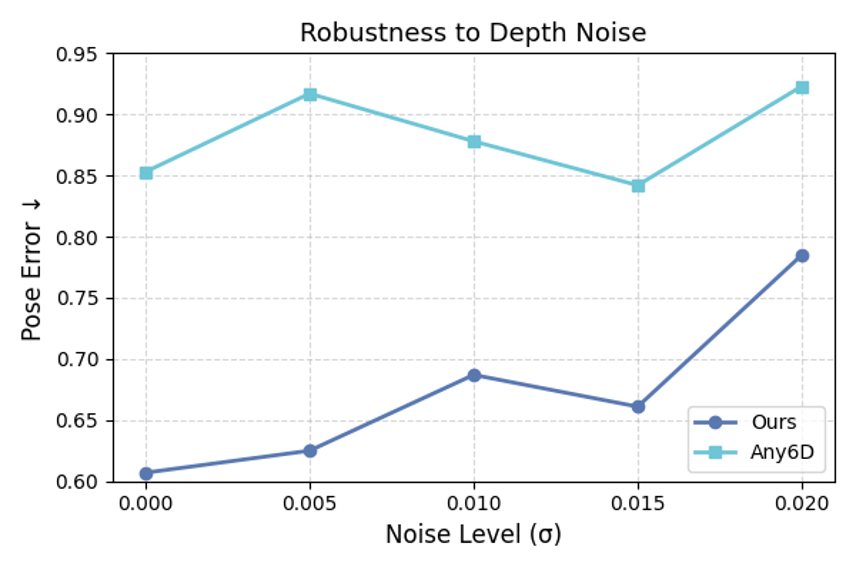
\includegraphics[width=1\linewidth]{depth_noise}
	\caption{Verification of the robustness of our method under deep noise.}
	\label{Fig. 5}
\end{figure}

 \bibliographystyle{IEEEtran}
 \bibliography{IEEEabrv,ral}

\end{document}


